\chapter{FREEFLOW}
\label{ff}
In this chapter we discuss the Freeflow programmable virtual switch
implementation details. The first few sections describe the higher level
components in this architecture, the control and data planes, applications, as
well as the virtual machine. Then we dive into the details of the object
models (e.g. ports, tables, and the packet context), native instruction
execution, as well as the memory and threading models currently supported.

\begin{figure}[h]
\centering
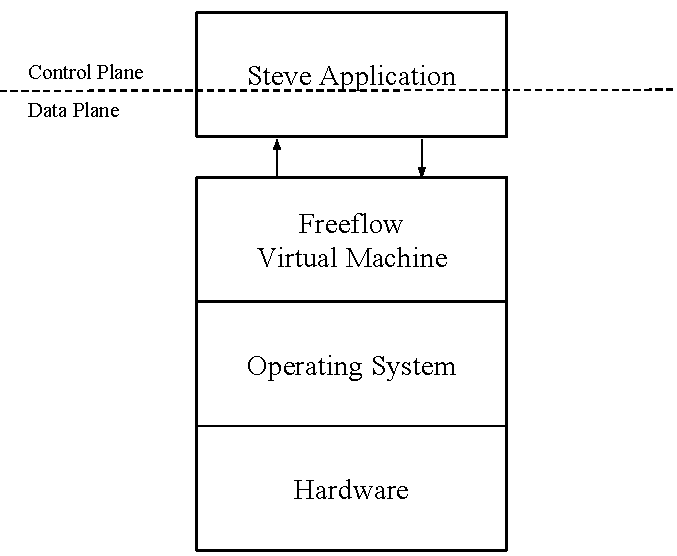
\includegraphics[scale=0.5]{ff_arch}
\caption{The Freeflow System Architecture.}
\label{ff_arch}
\end{figure}

\section{Control Plane}
\label{ff:cp}
The control plane acts as the brain in a network switch, and is responsible for
the hosting of applications as well as the management of the underlying data
plane. In the control plane, the system configuration establishes the resources
that must be provided to support application execution. During execution,
events raised from the data plane are caught and processed by application
defined event handlers in the controller.

\section{Data Plane}
\label{ff:dp}
A data plane executes the forwarding behavior for traffic flows using a variety
of hardware, and sometimes software, constructs available in a given system.

\section{Applications}
\label{ff:app}
Freeflow applications provide the logic for the control and data planes in the
switch. This is a departure from common SDN paradigms, where the two planes are
treated as separate entities and communicate over a secure channel. The reason
for blurring the line between the two parts is to reduce the overhead penalty
that is incurred in the former model. By allowing the application to straddle
the line between the control and data planes, the logic it provides is able
to be pushed into hardware and executed natively.

\begin{figure}[h]
\centering
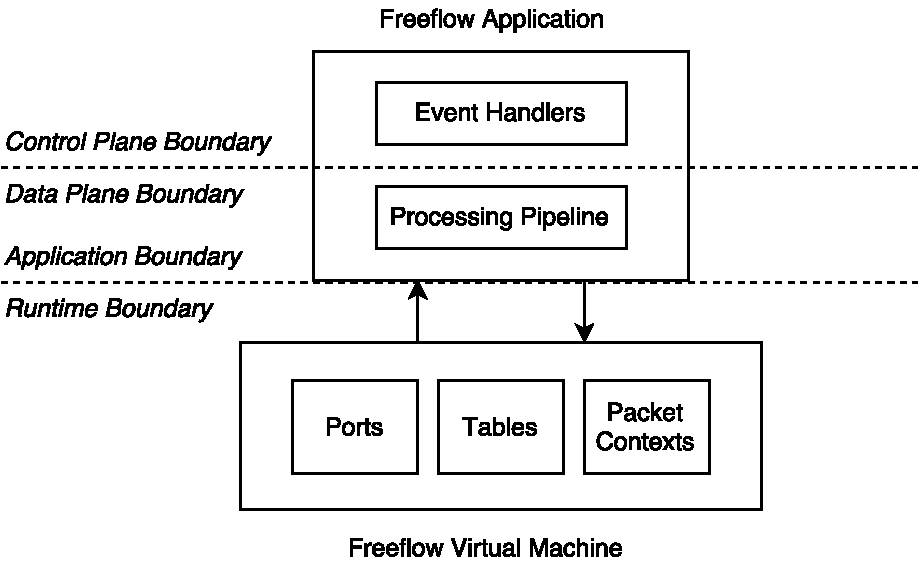
\includegraphics[scale=0.5]{application}
\caption{Freeflow application logic spans across the control and data plane
boundaries. Computational and memory resources are provided by the virtual
machine.}
\label{app}
\end{figure}

Networking applications operate on packets, utilizing information found inside
of nested protocol headers to determine the appropriate action to take. In
Freeflow, applications and the virtual machine operate on packet contexts,
which store meta data about a packet in the system. Applications use these
contexts generated by the system to perform protocol decoding and rule
matching logic as defined by the programmer. A typical application pipeline is
illustrated in Figure \ref{app_pipeline}.

\begin{figure}[h]
\centering
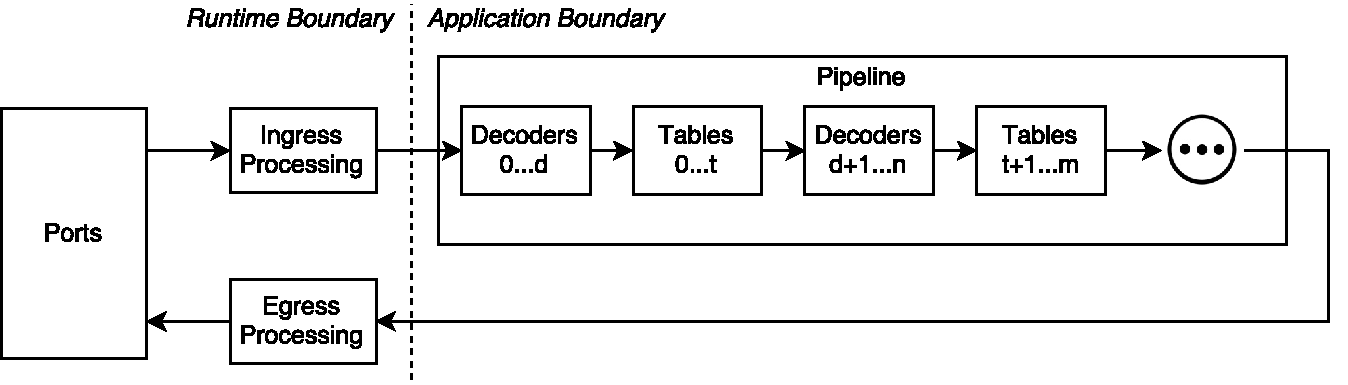
\includegraphics[scale=0.5]{app_pipeline}
\caption{A Freeflow application defines a list of decoders and tables.
Each decoder extracts values from a packet which are used in table lookups.}
\label{app_pipeline}
\end{figure}

\section{Packet Context}
\label{vm:packet-context}
Network packets are arranged as nested protocol headers, which contain fields
that describe the structure and contents of a particular layer. Since the
Freeflow data plane has no knowledge of any protocol structures (i.e. it is
protocol independent), it operates on contextual information extracted by
applications and stored in a \emph{context} object. The meta data contained
in a context allows the data plane to provide robust network functionality
and execute a variety of network applications.

\subsection{Packets}
In networking, packets represent raw data that has been transmitted over some
media with protocol headers for each layer contained in the packet. Each header
gives information about the structure and state of the current protocol being
processed. Figure \ref{ipv4_eth_frame} shows an example Ethernet frame
(packet) containing an IP (v4) header.

\begin{figure}[h]
\centering
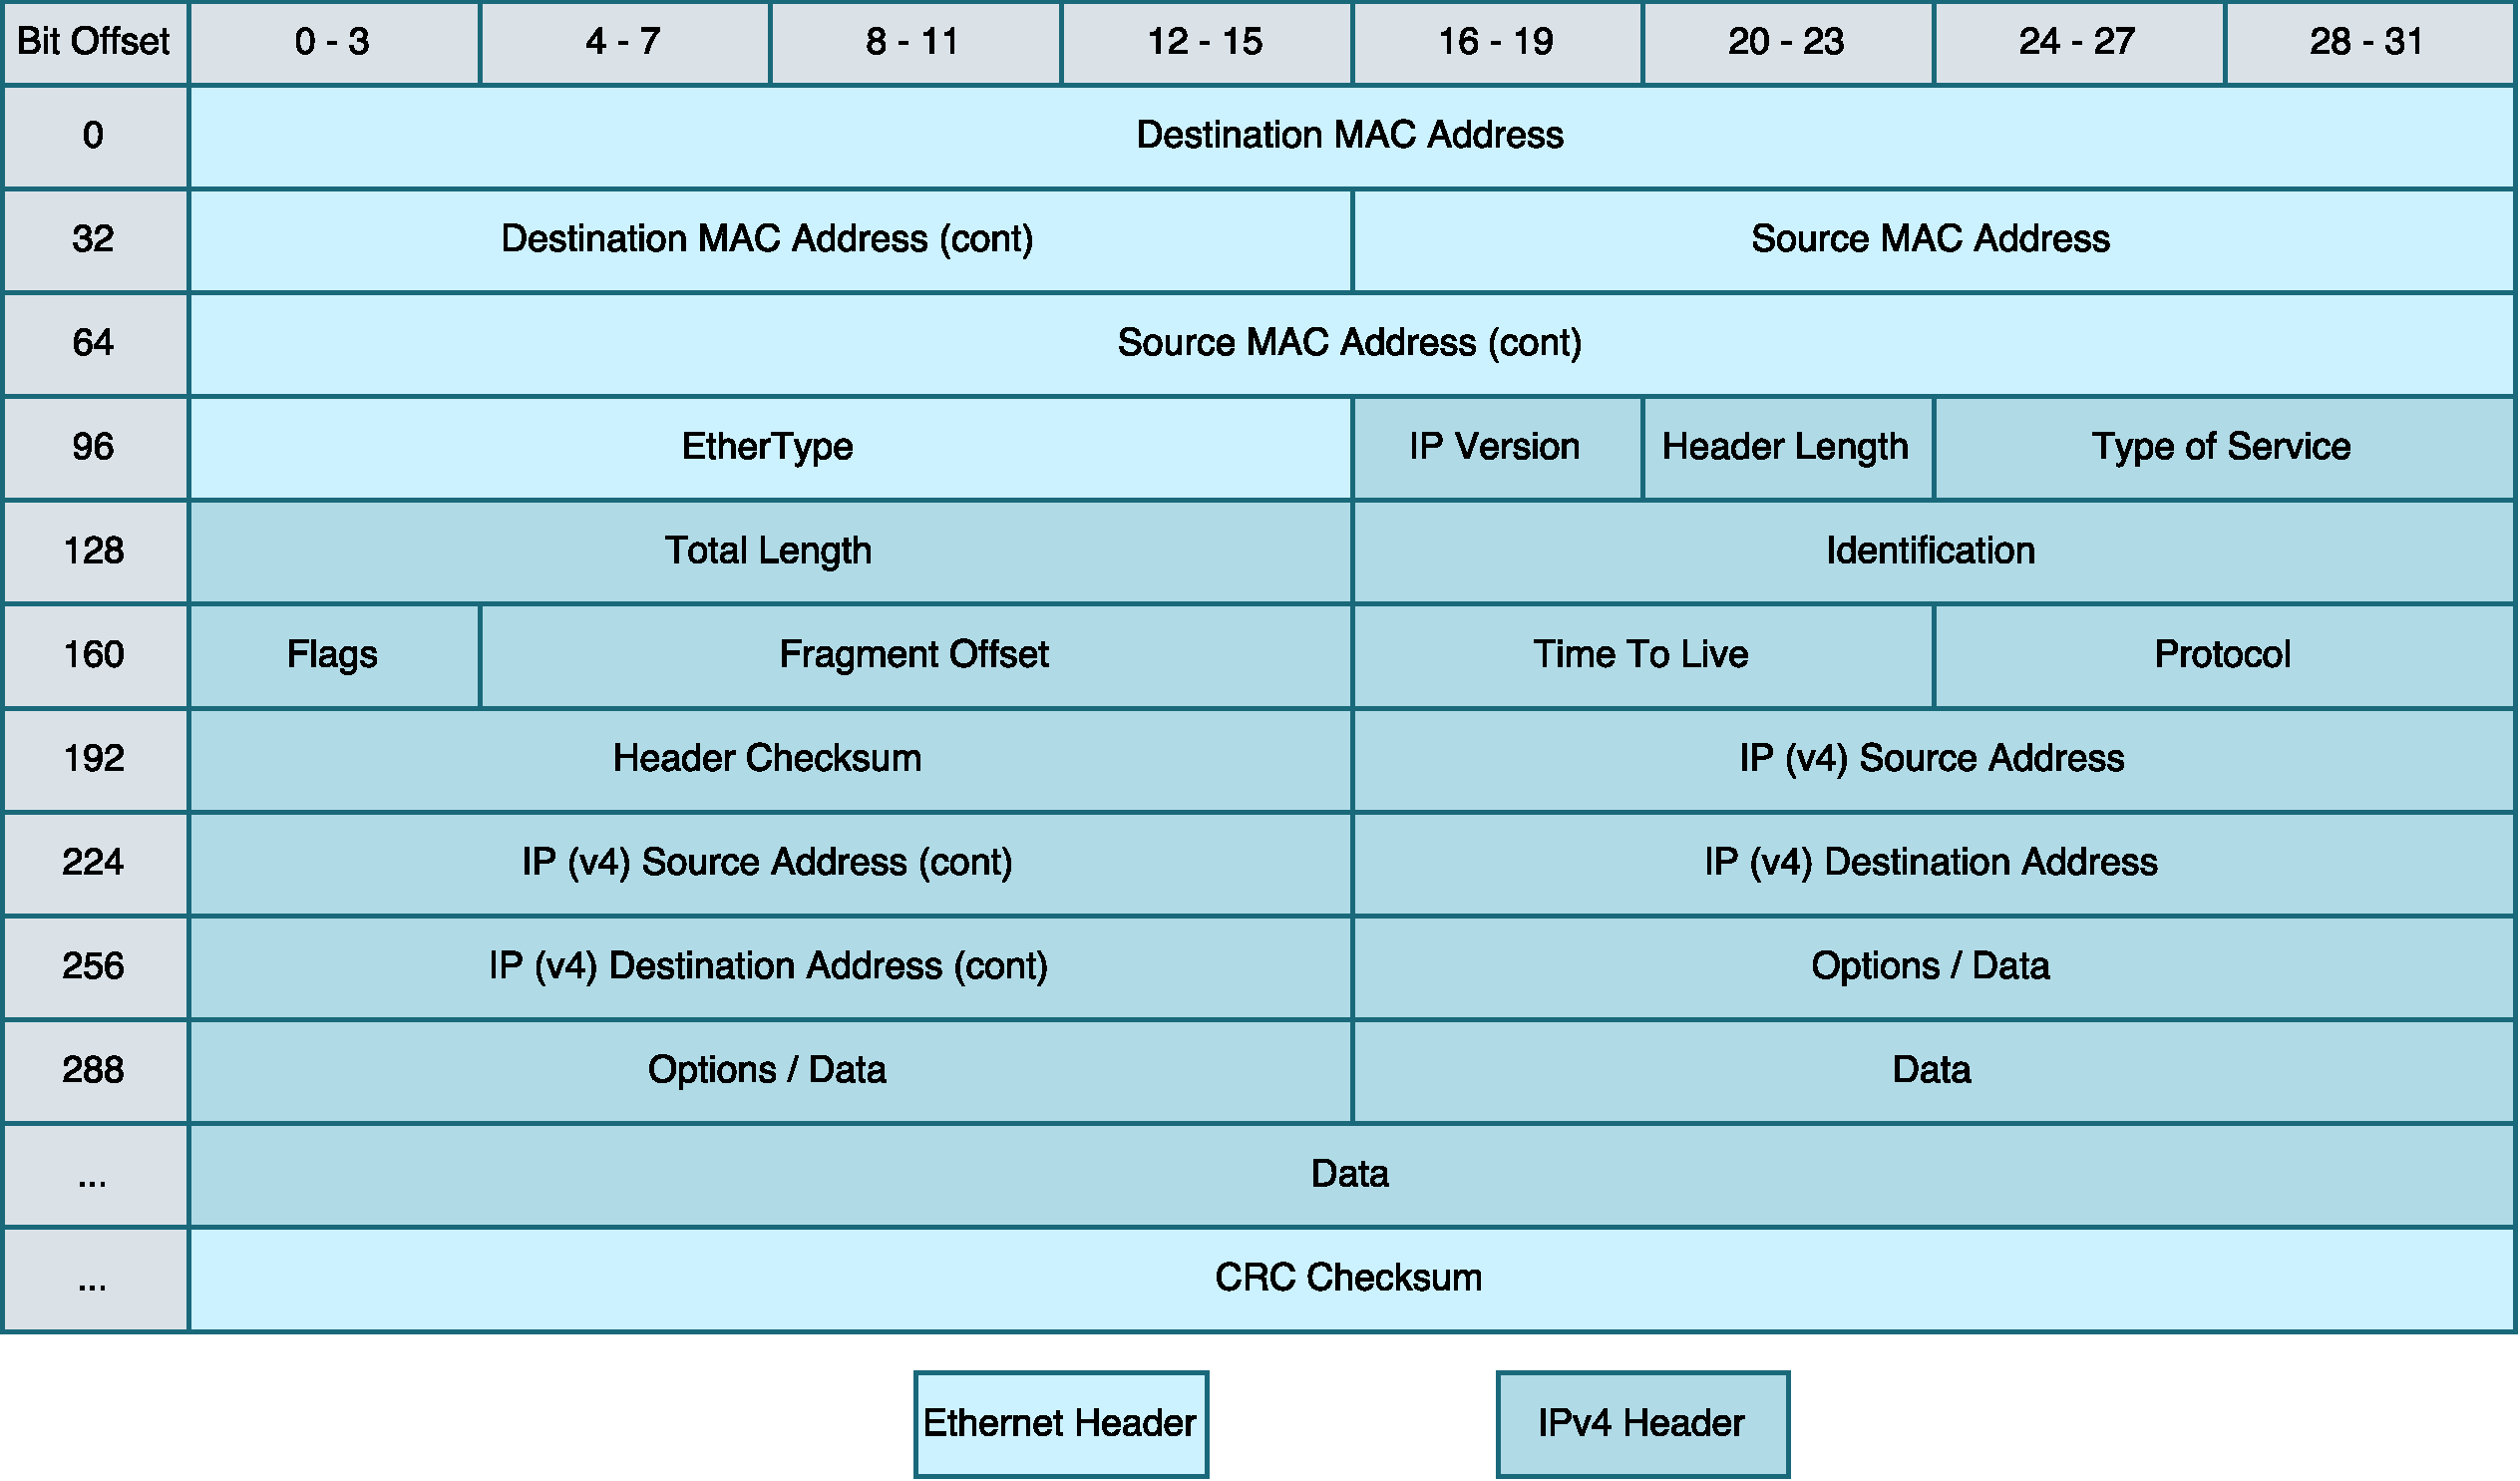
\includegraphics[scale=0.33]{ipv4_eth_frame}
\caption{An IPv4 Ethernet frame.}
\label{ipv4_eth_frame}
\end{figure}

The layout for each protocol is far from uniform, and fields within headers do
not always align to the traditional byte-aligned boundaries (e.g. Ethernet
MAC addresses which have a width of 48 bits). Storing these values in memory
results in wasted space, as larger data structures would need to be utilized.
Structure packing pragmas and bit width specifiers can be used to overlap
memory regions when the desired bit width is less than the standard width for
that type (e.g. \lstinline{std::uint_64 : 48;}). However storing a copy of the
packet data would result in coherency issues, negatively impacting
performance. Instead the fields within headers are stored in a \emph{binding
environment}, discussed in the following section.

\subsection{Context}
The packet \emph{context} provides contextual information about an associated
packet in the system. This is where applications store input, control, and
decoder information, as well as application metadata and build action lists.
Input information consists of data about the packets arrival into the system,
such as the input logical and physical ports. The control information maintains
the control flow of a context as it traverses processing pipelines.

\lstset{basicstyle=\tiny}
\begin{lstlisting}[language=c++]
struct Decode_info {
  uint16_t    pos;     // Packet decoding offset
  Environment headers; // Saved packet header locations
  Environment fields;  // Saved packet fields locations
};

struct Context {
  Ingress_info input;
  Control_info ctrl;
  Decode_info  decode;
  Packet       packet;   // A handle to packet memory
  Metadata     metadata; // Application-defined metadata
  Action_list  actions;  // A sequence of instructions
};
\end{lstlisting}

As application packet decoders execute, they store the position, or offset, and
length of the desired fields as pairs in a binding environment, referred to as
the decode information. This environment notes the offset of a field within the
current protocol header, as well as the offset for each protocol header within
the packet buffer. Utilizing this heavy weight approach to referencing protocol
field information ...

\begin{figure}[h]
\centering
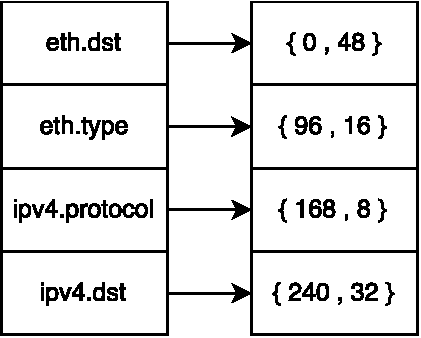
\includegraphics[scale=0.5]{context_concrete}
\caption{An example binding environment for an IPv4 Ethernet frame.}
\label{context_binding}
\end{figure}

\section{Virtual Machine}
\label{vm}
The Freeflow Virtual Machine is composed of modular parts that a programmer can
assemble into a virtual switch.

\begin{figure}[h]
\centering
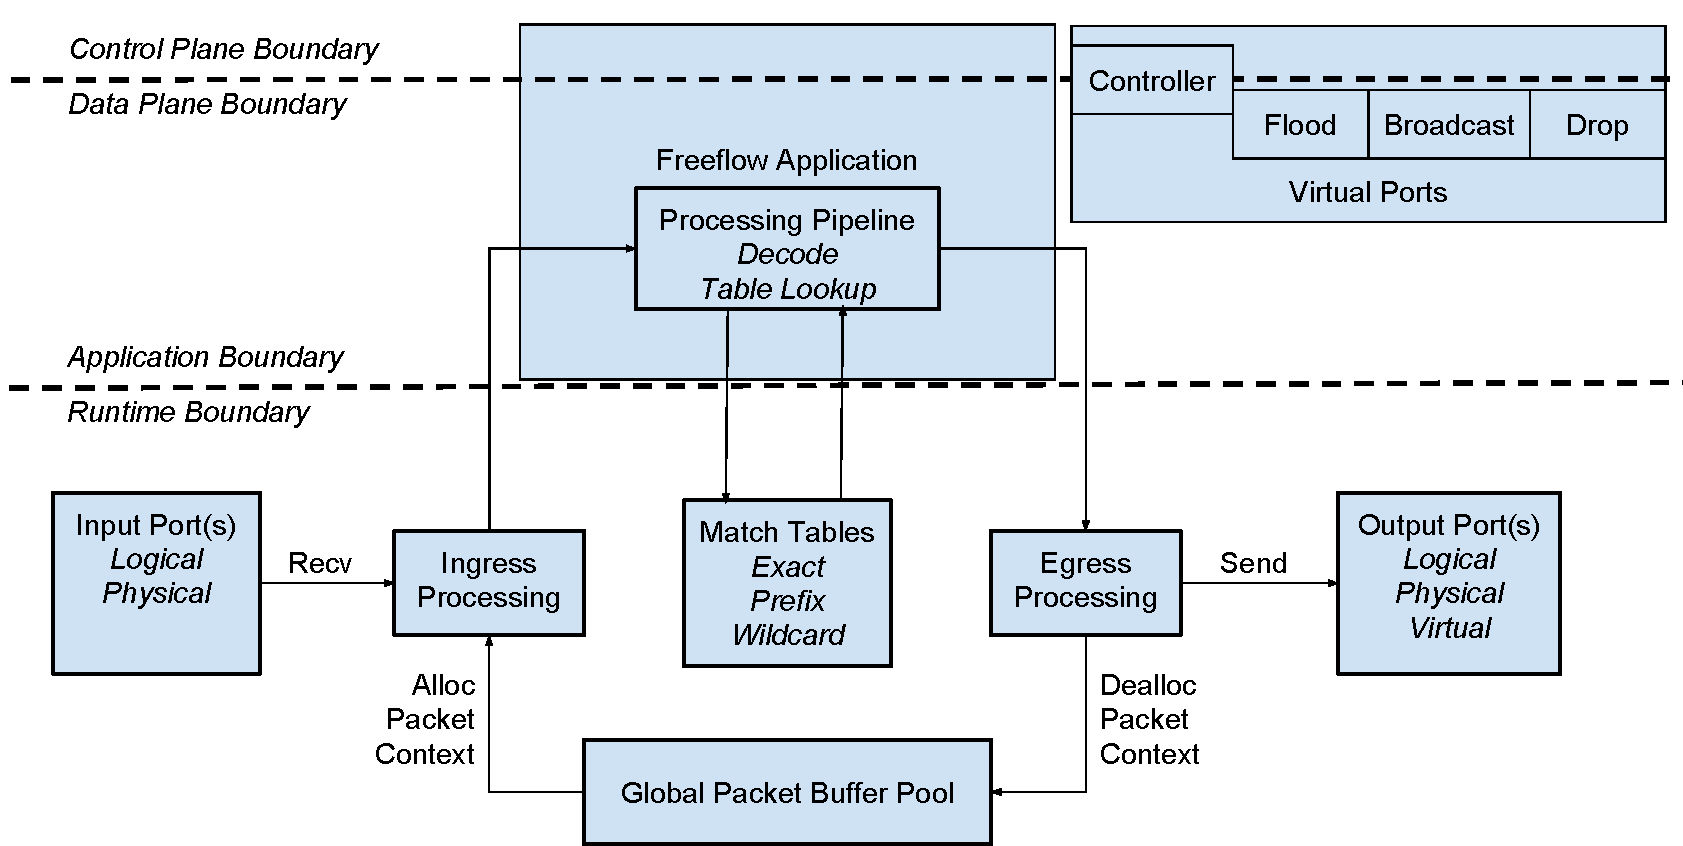
\includegraphics[scale=0.5]{ff_system}
\caption{The Virtual Machine System Architecture}
\label{ff_system}
\end{figure}

\section{Ports}
\label{vm:port}
Ports act as the main source of I/O for network applications. They provide the
means to receive and send packets that are entering and leaving the system. As
an abstract type, the port interface is fairly simple. Any derived port object
needs only implement the following four functions:

\begin{itemize}
\item Send - Transmit packet data.
\item Receive - Retrieve packet data.
\item Up - Puts the port into a usable state, data can be sent and received.
\item Down - Disables port functionality.
\end{itemize}

Port objects can be classified as being either physical, logical, or virtual. A
physical port represents a hardware networking interface, e.g. Ethernet cards.
Logical ports represent software networking constructs that utilize file
descriptors to act as a endpoint for communication. An illustration of the port
object UML can be found in figure \ref{port_uml}. Virtual ports are derived
from logical ports, and provide specialized functionality for the system. To
further classify the port type, they can be either seen as an \emph{input}
port, where data from an external source can be injected into the system, or an
\emph{output} port, which sends data to other external or internal devices.
Currently input ports can be either logical or physical, whereas output ports
can be any port type (i.e. logical, physical, virtual).

\begin{figure}[h]
\centering
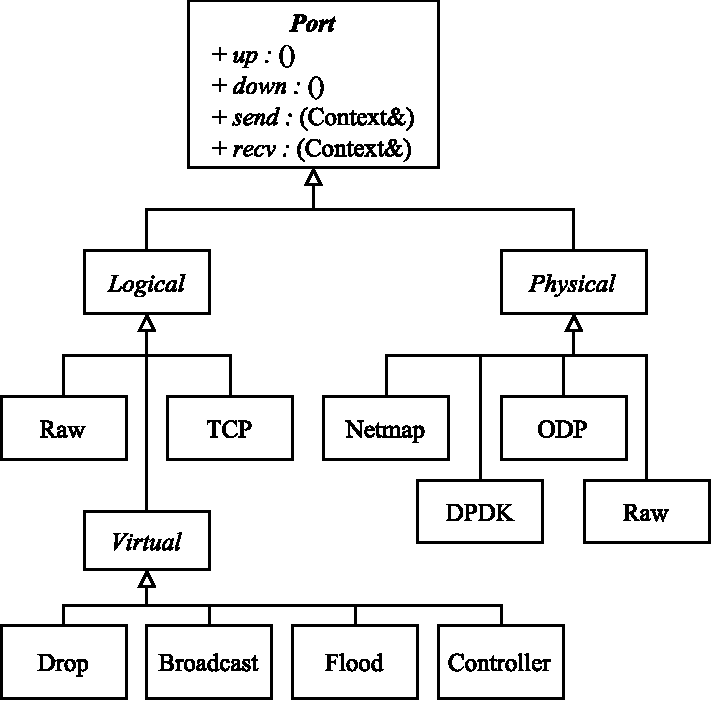
\includegraphics[scale=0.65]{ff_port_uml}
\caption{Freeflow port uml diagram.}
\label{port_uml}
\end{figure}

When packets are received by a port object, the memory that holds the raw
packet data and the context are allocated during this \emph{ingress} phase. The
underlying data store for the packet and context are owned and managed by the
port itself. Memory can be allocated from the ports internal resources (i.e.
memory mapped from a physical device address space) if present, or by the FFVM's
global buffer pool. This gives a greater amount of flexibility in that the
packet and context can exist in same memory region, potentially improving
locality. As packets leave the system during the \emph{egress} phase, this
memory is released back to the appropriate devices. Details about memory
management semantics can be found in section \ref{vm:memory}.

\section{Tables}
\label{vm:tables}
In network switches, tables are used to match properties of packets
with user-defined forwarding behaviors. They can be defined using a variety of
data structures and algorithms that implement them, but generally are categorized
as \emph{exact}, \emph{prefix}, or \emph{wild card}. All three table types are
currently implemented by the FFVM, though support for prefix and wild card is
incomplete.

% Insert table figure here.

Each entry in a flow table contains a \emph{key}, that is compared to a
certain field within packet. Key types vary between match table types. For an
exact match table the keys are integers of a set width, defined by the
application. These keys are used to aggregate traffic containing similar
characteristics into flows. Flows can be viewed as programs, or functions,
that get executed when a packet matches that their key. Each flow defines a
set of operations that are applied to packets.

% Another table figure here.

\section{Instructions}
\label{vm:insn}
Native insn execution. Offloading, optimizations.

\section{Memory}
\label{vm:memory}
Memory model.

\section{Threading}
\label{vm:threading}
Threading models.

\section{ABI}
\label{vm:abi}
What they can use.
